\chapter{ La Propuesta}

\section{Tipo y Diseño de la Investigación}

Esta investigación se clasifica como cuantitativa y descriptiva. El diseño corresponde a un estudio no experimental, ya que se analizan modelos de traducción automática existentes sin manipular variables, midiendo su impacto en la calidad semántica en un momento específico. El enfoque es comparativo utilizando muestreo no probabilístico de textos en quechua y análisis estadístico descriptivo para responder a los objetivos planteados.

\section{Proceso metodológico}
El proceso metodológico se estructura en cinco fases interrelacionadas:
\begin{itemize}
    \item Selección y preparación del corpus.
    \item Generación de traducciones automáticas
    \item Cálculo de métricas automáticas de calidad semántica*
    \item Evaluación humana de las traducciones
    \item Análisis comparativo de resultados    
\end{itemize}

\begin{figure}[htbp]
  \centering
  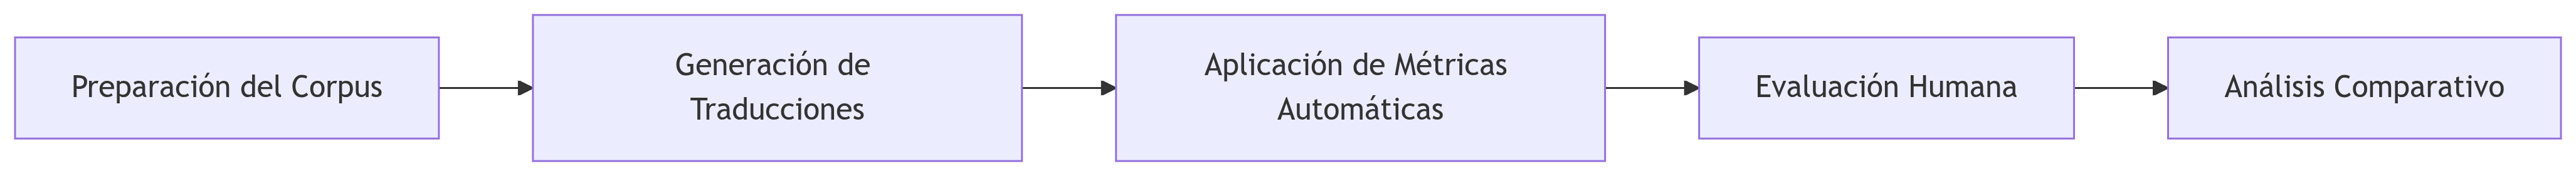
\includegraphics[width=0.95\textwidth]{figures/metodologia-fases.png}
  \caption{Fases de la evaluación de la calidad semántica de las TA quechua-español}
  \label{fig:mi_figura}
\end{figure}

    \section{Corpus de Estudio}
    
    El dataset empleado para este trabajo es el Monolingual Quechua IIC   \\
    \cite{zevallos2022}, que consta de 4,408,953
    tokens y 384,184 sentencias con variantes de quechua Collao y Chanka de la rama de Quechua II.
    Este corpus es una compilación de 50 corpus monolingües de diferentes fuentes y que abarco varios
    dominios como: religión, economı́a, salud, cultura, politica y misceláneos.
    
    \section{Modelos de traducción automática}
    
    Se evaluarán tres modelos de traducción automática representativos de distintos enfoques tecnológicos:

    \begin{table}[h!]
        \centering
        \caption{Comparación de modelos de traducción automática}
        \begin{tabularx}{\textwidth}{|X|X|X|}
        \hline
        \textbf{Modelo} & \textbf{Tipo} & \textbf{Implementación} \\
        \hline
        Google Translate & Comercial (Transformer multilingüe) & API pública \texttt{googletrans} \\
        \hline
        MarianMT & Especializado en lenguas minoritarias & Modelo \texttt{Helsinki-NLP/ opus-mt-quc-es} de Hugging Face \\
        \hline
        Baseline Léxico & Traducción basada en reglas & Diccionario quechua-español (Siminchik) + orden SVO \\
        \hline
        \end{tabularx}
        \label{tab:modelos_traduccion_tipo}
        \vspace{0.5cm}
        \textit{\textbf{Nota.} Elaboración propia.}
    \end{table}
    
        
    \section{Métricas de Calidad Semántica}
    
    Para la evaluación de calidad semántica, se emplean dos enfoques complementarios. El primero es un enfoque cuantitativo. Dentro de éste, se han establecido res métricas complementarias para evaluar la equivalencia semántica:

    \subsection{Similitud Coseno con LaBSE}
        \begin{itemize}
            \item \textbf{Objetivo:} Medir equivalencia conceptual global.
            \item \textbf{Fundamento técnico:} Representación vectorial en espacio semántico multilingüe.
            \item \textbf{Escala:} 0 (sin relación) a 1 (equivalencia total).
        \end{itemize}


        \begin{equation}
            \text{Similitud}(\mathbf{q}, \mathbf{t}) = \frac{\mathbf{q} \cdot \mathbf{t}}{\left\lVert\mathbf{q}\right\rVert \left\lVert\mathbf{t}\right\rVert}
        \end{equation}
 
        Donde:
        \begin{itemize}
            \item \textbf{q y t}: Vectores generados por \textit{LaBSE}.
            \item $\cdot$: Producto punto.
            \item $\left\lVert\mathbf{q}\right\rVert|$ y $\left\lVert\mathbf{t}\right\rVert|$: Normas Euclidianas de los vectores.
        \end{itemize}
    
    Esta métrica es particularmente relevante para capturar equivalencias no literales y adaptaciones culturales. 

    \subsection{COMET-QE (Quality Estimation)}
        \begin{itemize}
            \item \textbf{Objetivo:} Evaluar calidad intrínseca sin referencia humana
            \item \textbf{Fundamento técnico:} Modelo transformer preentrenado en evaluación de traducciones
            \item \textbf{Escala:} Puntuación continua (mayor valor indica mejor calidad)
        \end{itemize}

        \textbf{Fórmula (modelo Transformer):}

        \begin{equation}
        \text{COMET-QE} = f_{\theta}(\text{src}, \text{mt})
        \end{equation}
        
        Donde \( f_{\theta} \) es un modelo preentrenado que estima la calidad mediante:
        
        \begin{equation}
        f_{\theta} = \text{TransformerEncoder}(\text{Embed}(\text{src}) \oplus \text{Embed}(\text{mt}))
        \label{eq:Comet QE}
        \end{equation}
        
        
    \subsection{chrF++}
        \begin{itemize}
            \item \textbf{Objetivo:} Evaluar precisión léxica y morfológica
            \item \textbf{Fundamento técnico:} N-grams de caracteres adaptados a lenguas aglutinantes
            \item \textbf{Escala:} 0 a 1 (1 = máxima precisión)
        \end{itemize}

        \begin{equation}
        \text{chrF}_{++} = (1 + \beta^2) \cdot \frac{\text{chrP} \cdot \text{chrR}}{\beta^2 \cdot \text{chrP} + \text{chrR}}
        \end{equation}
        
        Donde:
        
        \begin{itemize}
          \item $\text{chrP}$: Precisión de n-gramas de caracteres (hasta 6-gram).
          \item $\text{chrR}$: Recall de n-gramas de caracteres.
          \item $\beta$: Peso para el recall (usualmente $\beta = 2$).
        \end{itemize}

    \subsection{Evaluación Humana}
  
    Paralelamente, se realiza una evaluación humana con cinco hablantes bilingües que califican fluidez (gramaticalidad y naturalidad) y adecuación (preservación de significado cultural) mediante escalas Likert, analizando 30 frases por modelo para identificar discrepancias entre métricas automáticas y percepción nativa.
    
    
    \section{Análisis de Datos}
    En el análisis de datos se emplearán varios enfoques para evaluar y comparar los resultados obtenidos de los diferentes modelos de traducción automática. Para la \textbf{comparación entre modelos}, se aplicará un \textbf{ANOVA unidireccional}, con el objetivo de identificar si existen diferencias significativas entre los promedios de los modelos evaluados. Posteriormente, se realizarán \textbf{pruebas post-hoc de Tukey} para realizar comparaciones más detalladas entre los pares de modelos, a fin de determinar cuáles son los modelos que presentan diferencias significativas. En todas estas pruebas, el \textbf{nivel de significancia} se establecerá en \textbf{$p < 0.05$}, lo que indicará si los resultados son estadísticamente significativos.

       
    En cuanto a la \textbf{correlación entre las métricas automáticas y las evaluaciones humanas}, se utilizará el \textbf{coeficiente de correlación de Pearson} para medir la relación entre los resultados obtenidos a través de las métricas automáticas y las evaluaciones realizadas por los evaluadores humanos. Además, se generarán \textbf{diagramas de dispersión} para visualizar de forma gráfica la relación entre las métricas y las evaluaciones por cada métrica, lo que permitirá identificar patrones o inconsistencias en las evaluaciones.
    

    
